% Created 2011-03-09 Wed 23:43
\documentclass[11pt,xcolor=svgnames]{beamer}

      \mode<presentation>

      \usetheme[height=12mm]{Rochester}
      \useinnertheme{umbcboxes}
      \useoutertheme{umbcfootline} 

      \usecolortheme{whale}

      \usefonttheme{structurebold}

%\usebackgroundtemplate{\includegraphics[width=\paperwidth]{format/libresoft-bg-soft.png}}
      %\beamertemplateballitem

      \setbeameroption{show notes}
      \usepackage[utf8]{inputenc}

      \usepackage[T1]{fontenc}

      \usepackage{hyperref}

      \usepackage{color}
      \usepackage{listings}
      \lstset{numbers=none,language=[ISO]C++,tabsize=4,
  frame=single,
  basicstyle=\small,
  showspaces=false,showstringspaces=false,
  showtabs=false,
  keywordstyle=\color{blue}\bfseries,
  commentstyle=\color{red},
  }
\setbeamertemplate{blocks}[rounded][shadow=true]
\setbeamertemplate{navigation symbols}{}

      \usepackage{verbatim}

      %\institute[xx]{<isra@herraiz.org>}

       %\subject{}

\usepackage[utf8]{inputenc}
\usepackage[T1]{fontenc}
\usepackage[english]{babel}
\usepackage{fixltx2e}
\usepackage{graphicx}
\usepackage{longtable}
\usepackage{float}
\usepackage{wrapfig}
\usepackage{soul}
\usepackage{textcomp}
\usepackage{marvosym}
\usepackage{wasysym}
\usepackage{latexsym}
\usepackage{amssymb}
\usepackage{hyperref}
\usepackage{listings}
\lstset{breakatwhitespace=true,
language=SQL,
columns=fullflexible,
keepspaces=true,
breaklines=true,
tabsize=3, 
showstringspaces=false,
extendedchars=true,
frame=none}



\tolerance=1000
\providecommand{\alert}[1]{\textbf{#1}}
%\DeclareGraphicsExtensions{.pdf,.png,.jpg}
\title{Starting a career in data science}
\author{Israel Herraiz}
%\date{}


\begin{document}

\maketitle

\begin{frame}
  \frametitle{Contents}
  \tableofcontents
\end{frame}



\AtBeginSection{
\begin{frame}
  \frametitle{}
  \tableofcontents[currentsection]
\end{frame}
}

\section{The Data Scientists}
\label{sec-1}

   
\begin{frame}[fragile]\frametitle{Why data science?}

  The intelligente use of data:
  \begin{itemize}
  \item has become a source of competitive advantage
    \begin{itemize}
    \item Better knowledge about the market
    \item Better knowledge about your customers
    \end{itemize}
  \end{itemize}

  \pause

  \begin{block}{The data science process}
    \begin{center}
      Data $\rightarrow$ Information $\rightarrow$ Decision
    \end{center}
  \end{block}

\pause

  \begin{exampleblock}{The goal}
    \centering \textcolor{blue}{\bf Data-Driven Decision Making}
  \end{exampleblock}
  
\end{frame}

\begin{frame}\frametitle{What is a data scientist?}
  \begin{block}{Key skills}
    \begin{itemize}
    \item Fitting in an \textcolor{blue}{\bf organization}, leading projects in a
      heterogeneous environment, aligning with strategy 
    \item Data-Analytic \textcolor{blue}{\bf Thinking}
    \item How to extract \textcolor{blue}{\bf knowledge} from data
    \end{itemize}
  \end{block}
  
  \begin{exampleblock}{The three facets of a data scientist}
    \begin{itemize}
    \item Functional (domain knowledge)
    \item Analytical (how to extract knowledge from data)
    \item Technical (how to implement the data science process)
    \end{itemize}
  \end{exampleblock}

  \pause

  \begin{alertblock}{Question}
    \begin{itemize}
    \item Are the three facets equally important? 
    \item Which facet is the most important?
    \end{itemize}
  \end{alertblock}
  
\end{frame} 

%% \begin{frame}\frametitle{Skills demanded in job postings}
%%   \begin{columns}[t]
%%     \begin{column}{0.45\textwidth}
%%       \begin{block}{Analytical skills}
%%         \begin{itemize}
%%         \item \textcolor{blue}{\bf Machine Learning}
%%         \item \textcolor{blue}{\bf Statistics}
%%         \item Bias towards engineering and scientific backgrounds
%%         \end{itemize}
%%       \end{block}
%%     \end{column}
%%     \begin{column}{0.45\textwidth}
%%       \begin{block}{Technical skills}
%%         \begin{itemize}
%%         \item \textcolor{blue}{\bf R} 
%%         \item \textcolor{blue}{\bf Python}
%%         \item \textcolor{blue}{\bf SQL}
%%         \item \textcolor{orange}{\bf Hadoop, Spark and Big Data} (covered only partially)
%%         \item Visualization technologies (\textcolor{blue}{\bf Tableau}, Qlik)
%%         \item Excel
%%         \end{itemize}
%%       \end{block}
%%     \end{column}
%%   \end{columns}
%% \end{frame}

\section{The Data Science Process}

\begin{frame}{The Data Science process}
  \begin{columns}[t]
    \begin{column}[t]{0.55\textwidth}
      \begin{block}{}
        \begin{center}
          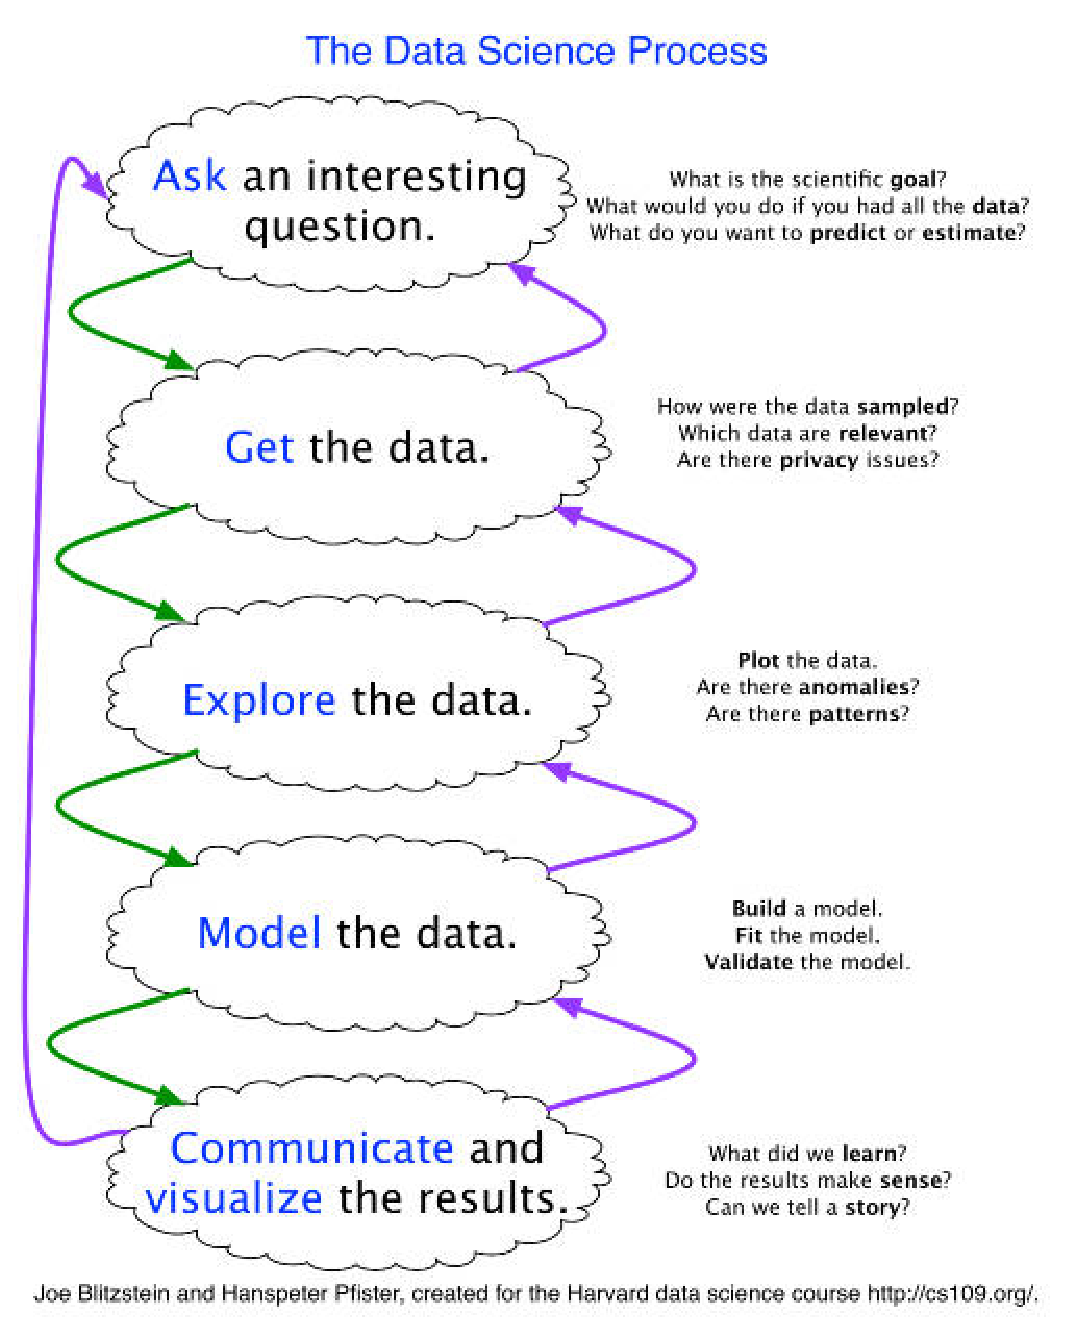
\includegraphics[scale=.3]{figs/data-science-process}
        \end{center}
      \end{block}
    \end{column}
    \begin{column}[t]{.4\textwidth}
      \begin{footnotesize}
        \begin{enumerate}
        \item Ask a question
          \begin{itemize}
          \item {\em \scriptsize Domain expertise}
          \end{itemize}
        \item Get and prepare the data
          \begin{itemize}
          \item {\em \scriptsize Python, Pandas, R}
          \end{itemize}
        \item Explore the data
          \begin{itemize}
          \item {\em \scriptsize Pandas, Matplotlib, R, Spark, Tableau}
          \end{itemize}
        \item Model the data
          \begin{itemize}
          \item {\em \scriptsize Python Scikit-Learn, R, Spark}
          \end{itemize}
        \item Communicate the results
          \begin{itemize}
          \item {\em \scriptsize Tableau, Looker}
          \end{itemize}
        \end{enumerate}
      \end{footnotesize}
    \end{column}
  \end{columns}
  \begin{tiny}
    \url{http://www.kdnuggets.com/2016/03/data-science-process-rediscovered.html}
  \end{tiny}

\end{frame}

\begin{frame}{But it is always iterative...}
  \begin{block}{Very rarely (never?) you will do it in just one pass}
    \begin{center}
      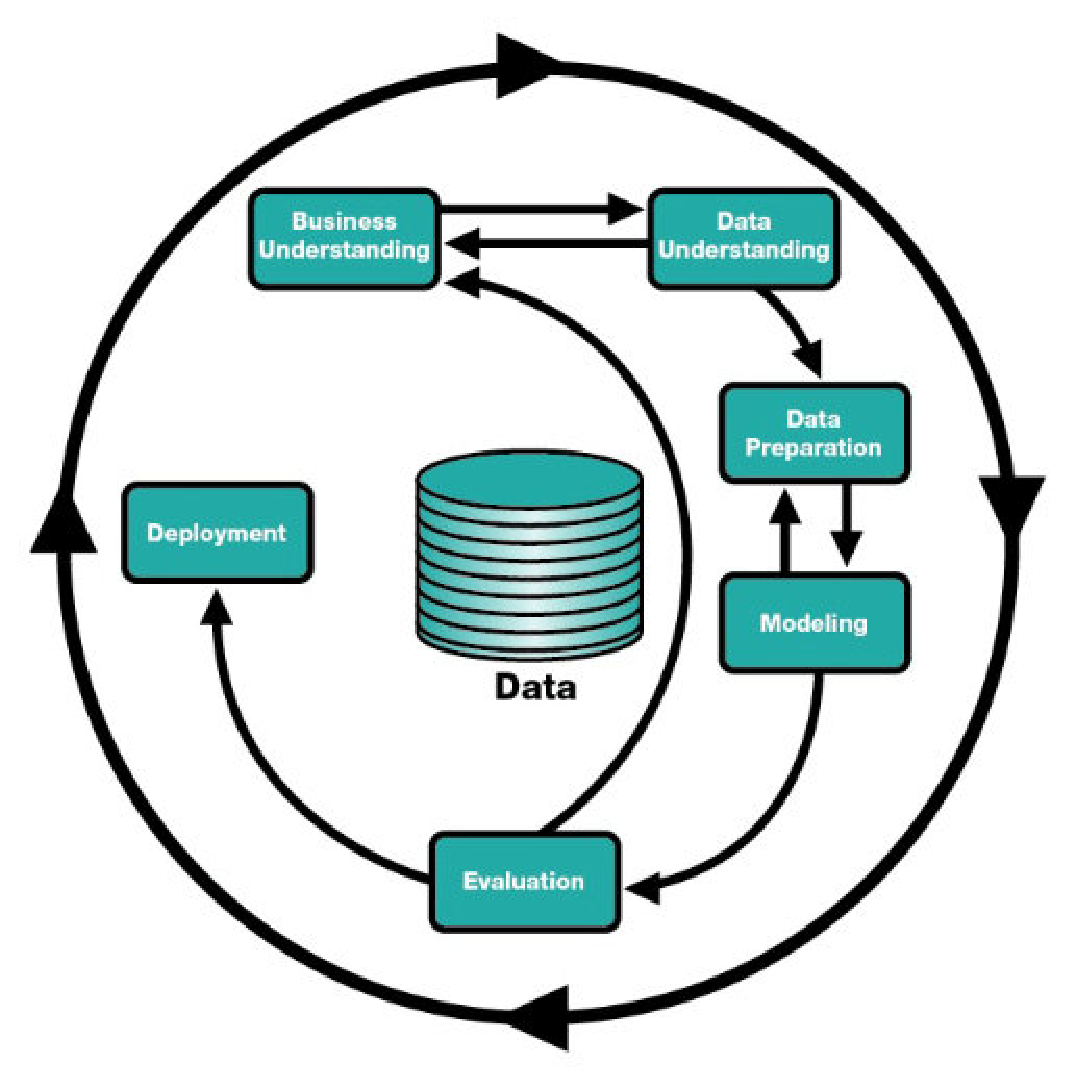
\includegraphics[scale=.35]{figs/crisp-dm}
    \end{center}
  \end{block}
  \begin{tiny}
    \url{https://en.wikipedia.org/wiki/Cross_Industry_Standard_Process_for_Data_Mining}
  \end{tiny}
\end{frame}

\begin{frame}{What kind of questions can we answer to?}
  \begin{block}{Machine Learning \& Statistics Applications}
    \begin{center}
      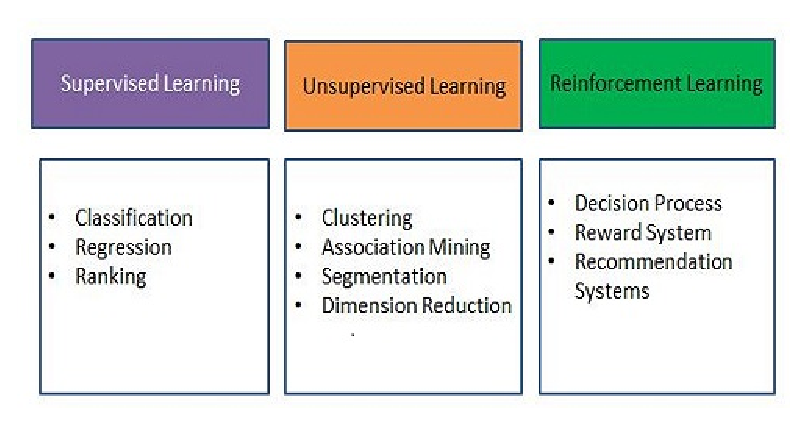
\includegraphics[scale=.75]{figs/machine-learning-applications}
    \end{center}
  \end{block}
  \begin{tiny}
    \url{http://www.kdnuggets.com/2015/09/questions-data-science-can-answer.html}
  \end{tiny}
\end{frame}

\begin{frame}{What kind of questions can we answer to?}
  \begin{block}{Classifications of questions}
    \begin{itemize}
    \item Is this $A$ or $B$?
      \begin{itemize}
      \item Binary classification
      \end{itemize}
    \item Is this $A$, $B$, $C$ or $D$?
      \begin{itemize}
      \item Multi-class classification
      \end{itemize}
    \item Is this normal or weird?
      \begin{itemize}
      \item Anomalies detection
      \end{itemize}
    \item How much or how many?
      \begin{itemize}
      \item Regression
      \end{itemize}
    \item How is this data organized?
      \begin{itemize}
      \item Unsupervised learning
      \item Dimensionality reduction
      \end{itemize}
    \item What should I do now?
      \begin{itemize}
      \item Recommendation systems
      \end{itemize}
    \end{itemize}
  \end{block}
\end{frame}

%% \section{Program of the Master in Data Science}

%% \begin{frame}\frametitle{The (main) program}
%%   \begin{itemize}
%%   \item \textcolor{blue}{\bf Intro to data science}
%%     \begin{itemize}
%%     \item Setup environment, working with the command line, intro to
%%       Git
%%     \end{itemize}
%%   \item \textcolor{blue}{\bf Data analysis}
%%     \begin{itemize}
%%     \item Python for Data Analysis
%%     \item Intro to Statistical Programming (R)
%%     \end{itemize}
%%   \item \textcolor{blue}{\bf Machine Learning and Statistics} (R, Python)
%%     \begin{itemize}
%%     \item Including a brief introduction to {\bf Deep Learning}
%%     \end{itemize}
%%   \item \textcolor{blue}{\bf Big Data}
%%     \begin{itemize}
%%     \item Very brief intro to Hadoop and Spark, using Python
%%     \item First steps in Google Cloud Platform
%%     \end{itemize}
%%   \item \textcolor{blue}{\bf Visualization and Business Intelligence}
%%     \begin{itemize}
%%     \item Dashboards development with Tableau
%%     \item Brief intro to D3.js
%%     \end{itemize}
%%   \end{itemize}
%% \end{frame}

\section{Recommendations to follow the program}

%% \begin{frame}\frametitle{Recommended books}
%%   \begin{columns}[t]
%%     \begin{column}{0.32\textwidth}
%%       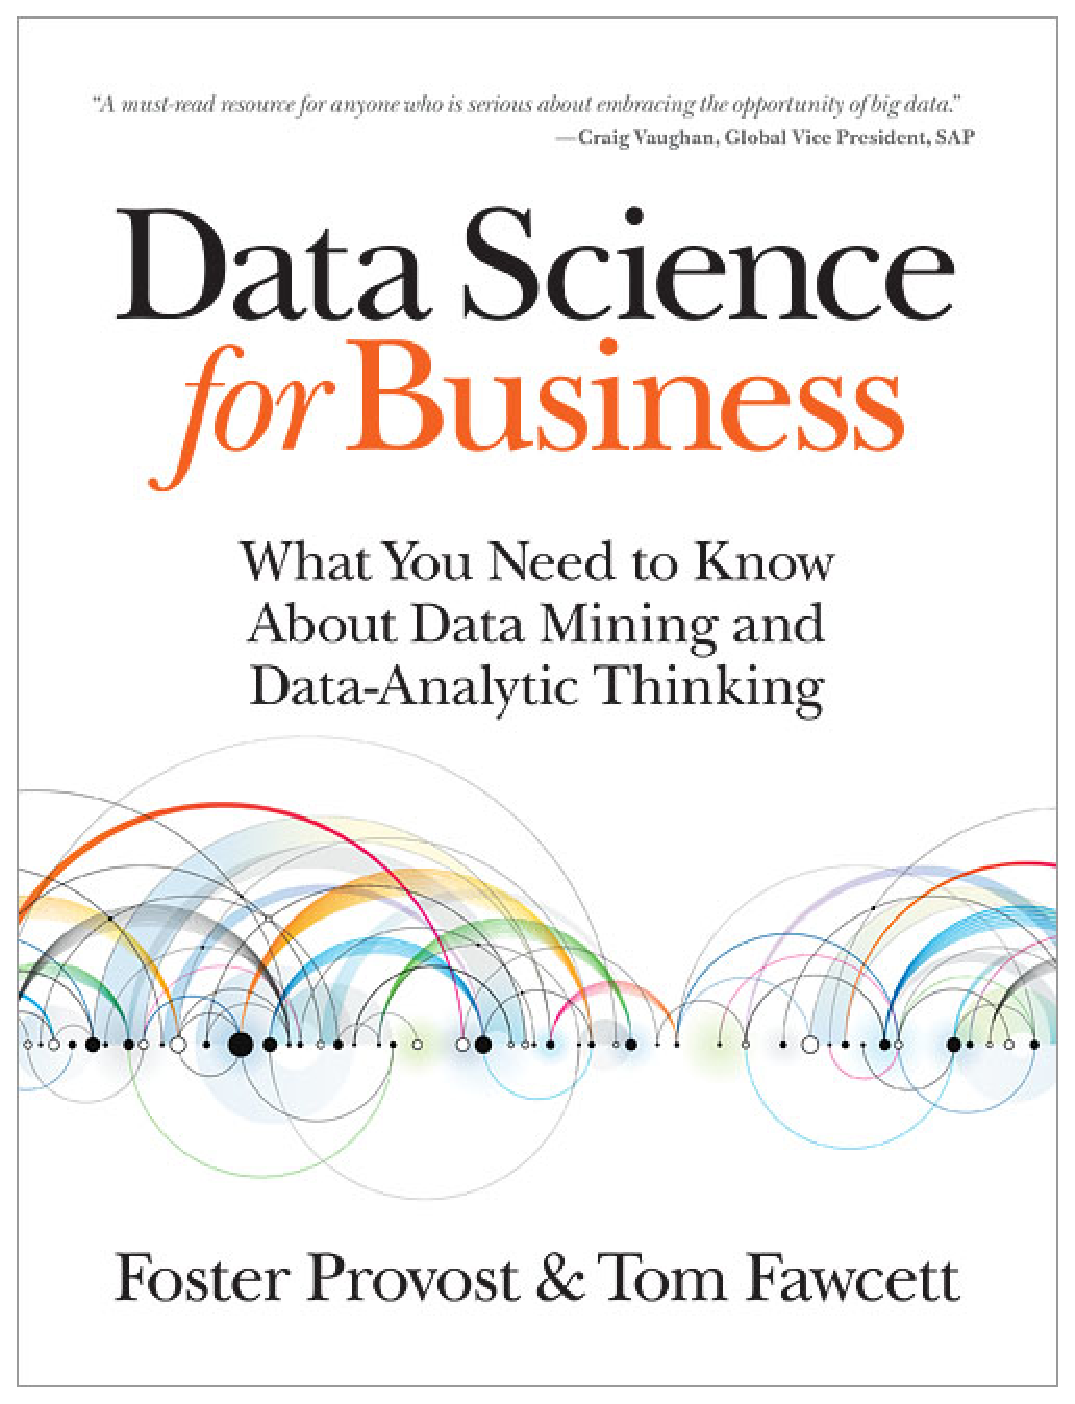
\includegraphics[scale=.2]{figs/data_science_for_business}
%%     \end{column}    
%%     \begin{column}{0.32\textwidth}
%%       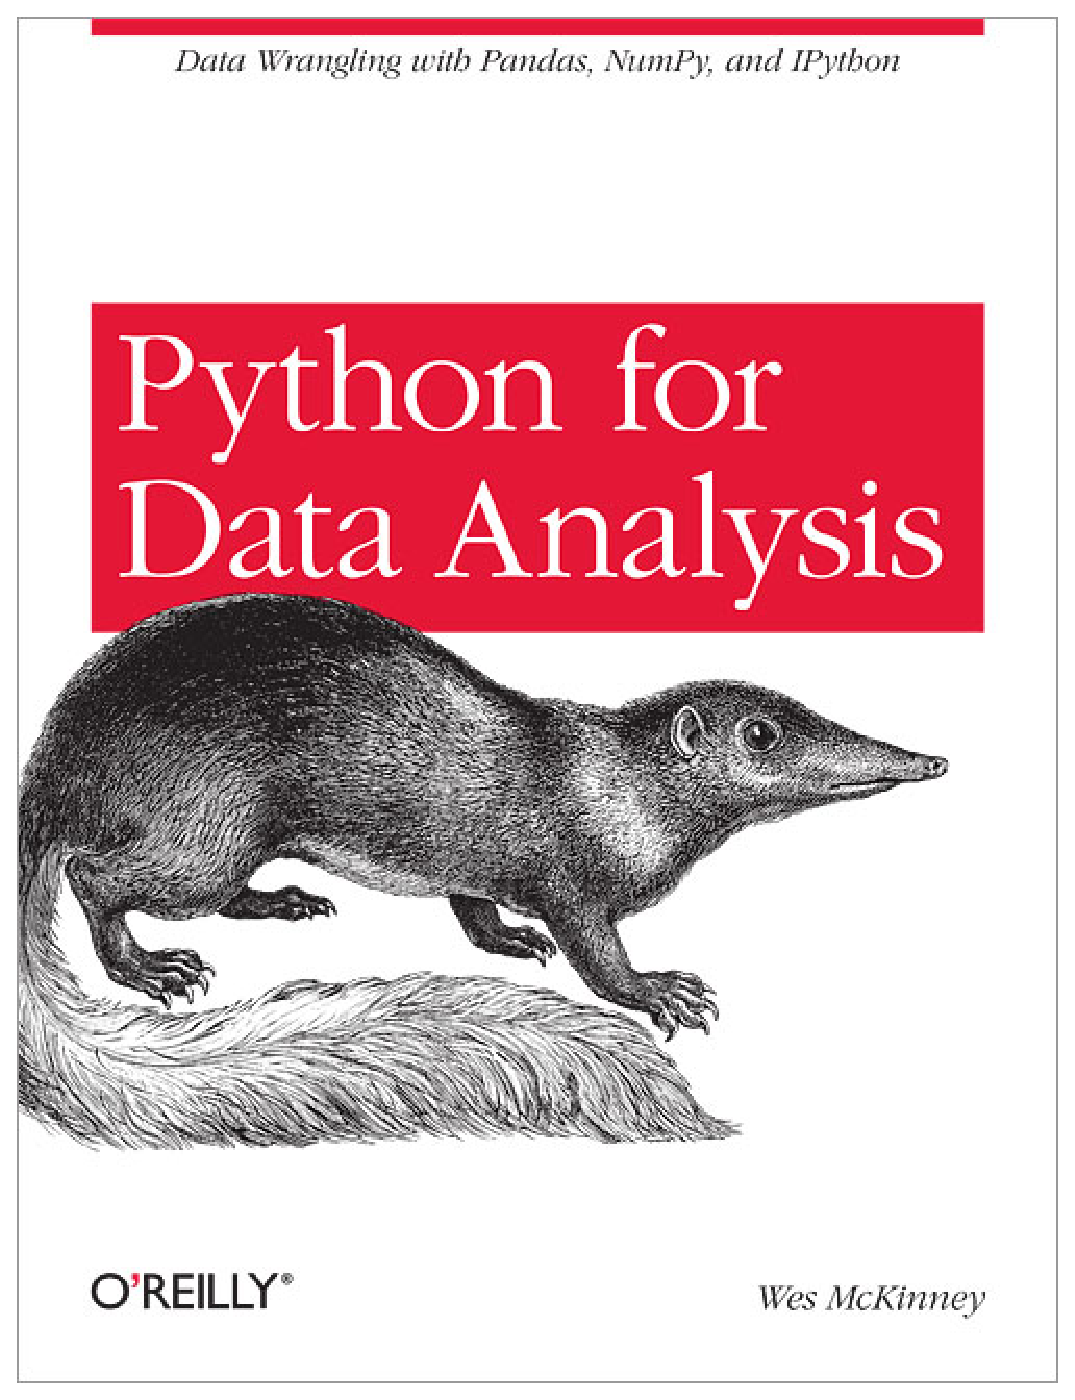
\includegraphics[scale=.2]{figs/python_for_data_analysis}
%%     \end{column}
%%     \begin{column}{0.32\textwidth}
%%       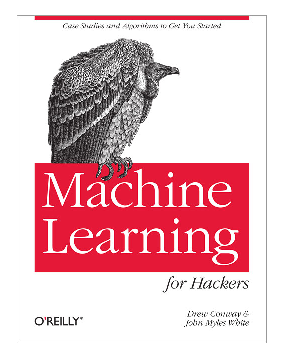
\includegraphics[scale=.85]{figs/machine_learning_for_hackers}
%%     \end{column}
%%   \end{columns}
%% \end{frame}

\begin{frame}\frametitle{Share promiscuously}
  \begin{block}{You need visibility}
    \begin{itemize}
    \item Use the social networks to position yourself as a data
      scientist
      \begin{itemize}
      \item \textcolor{red}{\bf Crucial:} Profile in
        \textcolor{blue}{\bf LinkedIn} and share, share, share!
      \item Share frequently about your progress in the master
      \end{itemize}
    \item Share your code in \textcolor{blue}{\bf Github} or Bitbucket
      \begin{itemize}
      \item Try to use it frequently, so it always shows recent
        activity
      \item Don't worry if you don't know Git, we will see in the
        first session
      \end{itemize}
    \item Don't mix (too much) your personal postings with your data
      scientist postings
      \begin{itemize}
      \item For instance, use Facebook for your personal network, and
        Twitter for your professional postings
      \end{itemize}
    \end{itemize}
  \end{block}
\end{frame}

%% \begin{frame}\frametitle{Recommended readings}
%%   \begin{block}{Amadeus Data Scientists series}
%%     \url{http://www.amadeus.com/blog/tag/data-scientist/}
%%   \end{block}

%%   \begin{block}{Gu\'ia de las profesiones de Internet}
%%     \url{http://www.avanzaentucarrera.com/llegaraser/profesiones-y-profesionales-de-internet}
%%   \end{block}
%% \end{frame}

\begin{frame}\frametitle{Take away}
  \begin{exampleblock}{Key ideas to remember}
\pause
    \begin{itemize}
    \item Extracting useful \textcolor{blue}{knowledge from data} to
      solve \textcolor{blue}{business problems} can be treated
      systematically by following a \textcolor{blue}{process} with
      reasonably \textcolor{blue}{well-defined stages}.
\pause
    \item From a \textcolor{blue}{large mass of data, information
        technology} can be used to \textcolor{blue}{find informative
        descriptive attributes} of entities of interest.
\pause
    \item If you look too hard at a set of data, you will find
      something -- but it \textcolor{blue}{might not generalize beyond} the
      data you are looking at.
\pause
    \item Formulating \textcolor{blue}{data science solutions} and
      evaluating the results involve thinking carefully about the
      \textcolor{blue}{context in which they will be used}.
\pause
    \item It's not about the technologies. Technology will always
      change very fast. \textcolor{blue}{Learn the concepts}, apply
      them with technology. \textcolor{blue}{Be open to learning} new
      technologies (and sometimes it will also imply learning new
      concepts). \textcolor{blue}{The only constant is change}.
    \end{itemize}
  \end{exampleblock}
\end{frame}

%% \section{This week's session}

%% \begin{frame}\frametitle{Program for this week}
%%   \begin{block}{Intro to data science}
%%     We have just completed this part.
%%   \end{block}
%% \pause
%%   \begin{block}{The environment}
%%     Setting up the environment
%%   \end{block}
%% \pause
%%   \begin{block}{Starting with Git}
%%     Intro to Git, and the importance of sharing our source code
%%   \end{block}
%% \pause
%%   \begin{block}{Getting familiar with the command line}
%%     Many times the shell command line is enough to answer to a lot of
%%     questions 
%%   \end{block}
%% \end{frame}

\end{document}
